\documentclass[12pt,a4paper]{article}
\usepackage[utf8]{inputenc}
\usepackage{graphicx}
\usepackage{amsmath}
\usepackage{amsthm}
\usepackage{amssymb}
\usepackage{hyperref}

\begin{document}

\begin{titlepage}
	\centering
	
\includegraphics[width=0.15\textwidth]{IIIT-B_logo.jpg}\par\vspace{1cm}
	{\scshape\LARGE International Institute of Information Technology Bangalore \par}
	\vspace{1cm}
	{\scshape\Large Project Proposal\par}
	{\Large DS/NC/ESD 863 Machine Perception\par}
	\vspace{1.5cm}
	{\huge\bfseries Vehicle Driving Assistant \par}
	\vspace{2cm}	   
	{\Large\itshape Akanksha Dwivedi - MT2016006\par}
	{\Large\itshape Anoop Toffy - MT2016016\par}
	{\Large\itshape Athul Suresh - MT2016030\par}
	{\Large\itshape Tarini Chandrashekhar - MT2016144\par}
	\vfill
	{\huge Group 7 \par}
	\vfill
	Guide : \par
	Prof. Dinesh Babu Jayagopi 

	\vfill

% Bottom of the page
	{\large \today\par}
\end{titlepage}


\tableofcontents
%\listoffigures
%\listoftables
\newpage

\section{Brief Description}
This project aims to provide a comprehensive set of assistance features to aid the driver (or autonomous vehicle) to drive safely. This includes a number of indicator and cues regarding the environment.  
\vspace*{1cm}
\subsection{Problem Formulation}
\begin{itemize}
\item[--] Application/System (Driving Assistance)
	\begin{itemize}
	\item[--] MP Module (Obstacle detection)
	\begin{itemize}
	\item[--] ML task (Multiclass Classification)
	\begin{itemize}
		\item[--] Features, Models, Optimization algorithm (To be decided based on empirical observations)
		\end{itemize}
	\end{itemize}
\end{itemize}						
\end{itemize}
\newpage
\section{Dataset}
360p video of roads in and around Electronic City Phase was recorded by us. We used a Cannon 1300D to record the video. 


\begin{figure}[!h]
\centering
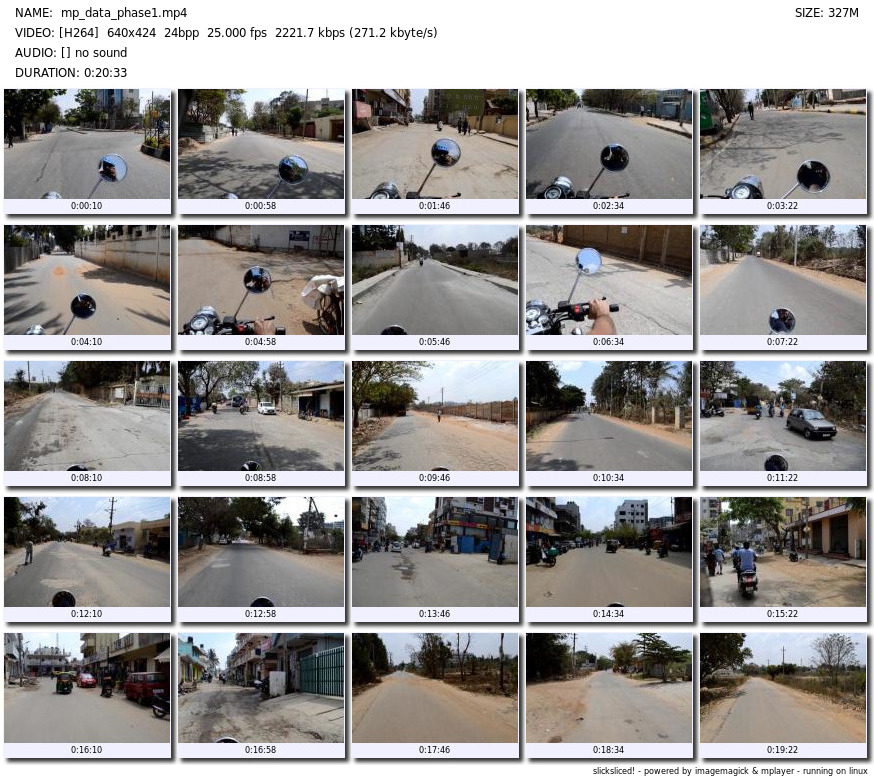
\includegraphics[width=1.0\textwidth]{datasets.jpg}
\caption{Dataset thumbnails}
\end{figure}

\newpage

\section{Proposed Plan of Execution}

\subsection{Phase 1}
\begin{itemize}
\item Data collection and video pre-processing.
\begin{quote}
Video of roads in Electronic City was collected manually with a DSLR camera held by a pillion rider on a moving motorcycle. About 20 minutes worth of video was collected for Phase 1 of the project. The video was pre-processed to reduce excessive jitter.
\end{quote}

\end{itemize}


\subsection{Phase 2} 
\begin{itemize}
\item Pothole detection in video frames.
\end{itemize}


\subsection{Phase 3}
\begin{itemize}
\item Improving accuracy of the current model.
\item Comparing the result with alternate models.
\end{itemize}


\subsection{Phase 4}
\begin{itemize}
\item Detection of other obstacles (pedestrians, oncoming traffic etc).
\item Provide driving cues based on detected entities. 
\end{itemize}



\section{Main Challenges}
\begin{itemize}
\item Procuring large and varied data to work on.

\item Presence of noise, shadows and excessive jitter in data.

\item Diversity and non-uniformity among roads and potholes which makes it difficult to generalise. 

\item Detecting obstacles with an obstructed field of view.

\item Consistency in object detection with increase in speeds.
\end{itemize}


\section{Learning Objectives}
\begin{itemize}
\item Finding a real world problem and formulating it as a machine perception problem.

\item Get acquainted with different aspects of image analysis for feature extraction.

\item Be able to extract appropriate features and apply machine learning algorithms to solve the problem.

\item Be able to read current research papers and understand the issues discussed.

\item Obtaining and cleaning data.
\end{itemize}

\end{document}